\section{Architecture du modèle}

Pour répondre à la problématique de la découverte de nouveaux matériaux donneurs pour les OSC, 
nous nous appuyons sur les travaux de \textbf{Jinyu Sun et al. \cite{Sun}} qui ont développé un modèle d'apprentissage profond pour la génération de molécules et du QuantumDeepField de \textbf{Masashi et al. \cite{Masashi}} capable de prédire les propriétés électroniques des molécules. 

\subsection{Modèle de prédiction de propriétés (PCE)}

Dans ce modèle, nous parlerons du \textbf{Quantum Deep Field} (QDF) pour prédire les propriétés des matériaux donneurs telles que le PCE.
L'architecture du modèle repose sur deux réseaux de neuronnes profonds majeures : le réseau de neurones de prédiction de propriétés et le réseau de neurones basés sur des contraintes physiques.
L'architecture du modèle est illustrée ci-dessous. \\


\begin{figure}[htbp]
    \centering
    \resizebox{\linewidth}{!}{
        \begin{tikzpicture}[ >=Latex,  % Pour les pointes de flèche
            line cap=round, line join=round,  % Bords arrondis
            wavefn/.style={thick}    % Style pour tracer les fonctions
        ]
        
        % (1) Le « M » stylisé et l'étiquette "Molecule"
        \node[font=\large] (M) at (0,0) {$\mathcal{M}$};
        \node[below=2pt of M] {Molecule};
        
        % (2) Grande flèche horizontale (à droite du M)
        \draw[thick,->] (1,-0.2) -- ++(7,0)
            node[midway, below=3pt]{Gaussian-type orbitals};
        
        % (3) Tracer les trois "orbitales" gaussiennes
        % Première orbitale φ1
        \begin{scope}[xshift=2.2cm, yshift=0cm]
            \draw[->] (0,0) -- (0,1.3);
            \draw[->] (0,0) -- (1.2,0);
            \draw[domain=0:1.0, samples=40, wavefn]
            plot (\x,{1.0*exp(-5*(\x)^2)});
            \node[above] at (0.5,0.8) {$\phi_1$};
        \end{scope}
        
        % Deuxième orbitale φ2
        \begin{scope}[xshift=3.9cm, yshift=0cm]
            \draw[->] (0,0) -- (0,1.3);
            \draw[->] (0,0) -- (1.2,0);
            \draw[domain=0:1.0, samples=40, wavefn]
            plot (\x,{1.0*exp(-5*(\x)^2)});
            \node[above] at (0.5,0.8) {$\phi_2$};
        \end{scope}
        
        % Troisième orbitale φ3
        \begin{scope}[xshift=5.6cm, yshift=0cm]
            \draw[->] (0,0) -- (0,1.3);
            \draw[->] (0,0) -- (1.2,0);
            \draw[domain=0:1.0, samples=40, wavefn]
            plot (\x,{1.0*exp(-5*(\x)^2)});
            \node[above] at (0.5,0.8) {$\phi_3$};
        \end{scope}
        
        % Étiquette "Atomic basis functions"
        \node[font=\Large] (phi) at (9,0) {$\mathcal{\phi}$};
        \node[below=2pt of phi] {Atomic basis functions};
        
        \draw[thick,->] (10,-0.2) -- ++(7,0)
            node[midway, below=3pt]{LCAO};
        
        % L'équation LCAO
        \node[above] at (13.5,0.1) {$\psi = c_{1}\phi_{1} + c_{2}\phi_{2} + c_{3}\phi_{3}$};
        
        \node[font=\Large] (psi) at (18,0) {$\mathcal{\psi}$};
        \node[below=2pt of psi] {Kohn-Sham molecular orbitals};
        
        \draw[->, thick] (18,-1) -- (18, -3.5) node[midway, left] {Squared sum};
        
        \node[font=\Large] (rho) at (18,-4) {$\mathcal{\rho}$};
        \node[below=2pt of rho] {Electron density};
        
        \draw[->, thick] (17,-4) -- (1, -4) node[midway, above] {Hohenberg-Kohn map};
        
        \draw[<-, thick] (17,-4) -- (1, -4) node[midway, below] {\drawNeuralNetwork{1,3,3,3,1}{1pt}{1cm}{0.9cm}};

        % External potential
        \node[font=\Large] (V) at (0,-4) {V};
        \node[below=2pt of V] {External potential};
        
        \draw[->, thick] (0,-1) -- (0, -3.5) node[midway, right] {Atomic numbers and Gaussian};
        
        \draw[->, thick] (19, -0.2) -- ++ (7, 0) node[midway, above] {Power conversion efficiency functional};

        \draw[->, thick] (19, -0.2) -- ++ (7, 0) node[midway, below] {\drawNeuralNetwork{3,3,3,1}{1pt}{1cm}{0.9cm}};
        
        \node[font=\Large] (PCE) at (27,0) {PCE};
        
        \draw[dashed, ->] ($(rho)+(1,0)$) -| (PCE);
        
        \end{tikzpicture}
    }
    \caption{Quantum Deep Field (QDF) pour la prédiction de PCE}
    \label{fig:architecture}
\end{figure}


% \paragraph{Étape 1 \: Représentation de la molécule } 
\subsubsection{Représentation de la molécule}
La molécule d’intérêt, notée $\mathcal{M}$, est d’abord représentée sous forme de coordonnées atomiques et de numéros atomiques. Cette représentation sert de point de départ pour la génération des fonctions de base atomiques.

% \paragraph{Étape 2 \: Construction des orbitales atomiques de type gaussien} 
\subsubsection{Construction des orbitales atomiques de type gaussien}
À partir de la structure moléculaire, des orbitales atomiques de type gaussien ($\phi_1$, $\phi_2$, $\phi_3$, ...) sont générées. Ces fonctions de base servent à décrire la distribution électronique autour de chaque atome.

\subsubsection{Combinaison linéaire des orbitales atomiques (LCAO)}
Les orbitales atomiques sont combinées linéairement pour former les orbitales moléculaires de Kohn-Sham ($\psi$), selon la méthode LCAO ($\psi = c_1\phi_1 + c_2\phi_2 + c_3\phi_3$). Cette étape permet de modéliser la structure électronique de la molécule.

\subsubsection{Densité électronique et HK\_map}
La densité électronique ($\rho$) est obtenue en sommant les carrés des orbitales moléculaires. Cependant, minimiser uniquement la fonction de perte $\mathcal{L}_{PCE}$ ne garantit pas que le modèle appris soit physiquement significatif. 

En effet, en raison de la forte non-linéarité du réseau de neurones profond (DNN), il est possible d'obtenir un PCE correcte même si les orbitales de Kohn-Sham $\psi$ ne sont pas valides. Cela signifie que le modèle ne garantit pas que les orbitales $\psi(\mathbf{r})$ produisent la bonne densité électronique $\rho(\mathbf{r}) = \sum_{n=1}^N |\psi_n(\mathbf{r})|^2$.

Pour remédier à ce problème, une contrainte supplémentaire est imposée sur $\psi(\mathbf{r})$ basée sur le théorème de Hohenberg-Kohn, qui assure que le potentiel externe $V(\mathbf{r})$ est une fonction unique de la densité électronique.

\subsubsection{PCE}
Le PCE est calculé à partir des orbitales moléculaires. Il est exprimé par un DNN, ce qui permet d'évaluer l'efficacité de conversion d'énergie de la molécule. \\

En somme, on a 2 prédictions princiaples effetuées par le modèle :
\begin{itemize}
    \item \textbf{Prédiction du potentiel $V(\mathbf{r})$} : La première, qui est une prédiction sur le potentiel,sert de contraintes physiques pour ajuster le modèle de prédiction de PCE.
    \item \textbf{Prédiction du PCE} : La deuxième prédiction est le PCE de la molécule.
\end{itemize}

\subsection{Modèle de genération de molécules}
Ce modèle repose sur une approche par modélisation générative utilisant
un Auto-Encodeur Variationnel (VAE), combinée à une préparation des
données chimiques. L'objectif est de créer un système capable de représenter
fidèlement les structures moléculaires dans un espace latent continu, puis d'utiliser
ces représentations pour générer de nouvelles structures prometteuses en termes
d'efficacité photovoltaïque

Le choix du VAE s'explique par sa capacité à encoder des données complexes dans
un espace latent structuré, tout en permettant la génération d'exemples nouveaux
par simple échantillonnage. Dans notre cas, cela permet de transformer des chaînes
SMILES en vecteurs continus, puis de régénérer des chaînes moléculaires viables à
partir de ces vecteurs. Le VAE est particulièrement utile pour éviter les erreurs
syntaxiques communes lors de la génération de nouvelles molécules.

Le modèle VAE utilisé dans ce projet se compose de trois parties principales :

\begin{itemize}
    \item \textbf{Encodeur} : transforme les SMILES vectorisés en une distribution latente gaussienne.
    \item \textbf{Espace latent} : échantillonnage dans cet espace pour produire des représentations moléculaires nouvelles.
    \item \textbf{Décodeur} : reconstruit des SMILES valides à partir des vecteurs latents.
\end{itemize}


\begin{figure}[H]
    \centering
    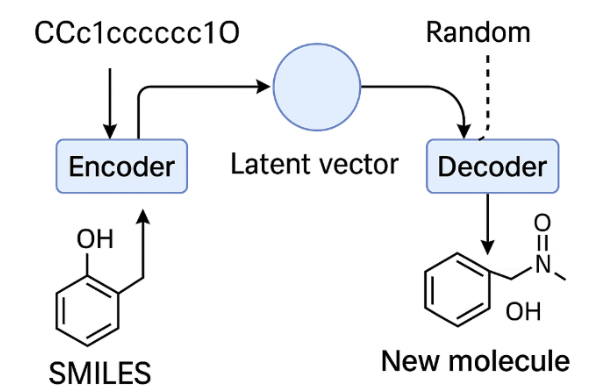
\includegraphics[width=0.4\textwidth]{Architecture/vae.png}
    \caption{Architecure VAE}
\end{figure}

Cette architecture permet non seulement de reproduire fidèlement les molécules du
dataset, mais aussi de générer des candidats inédits pour les OPV. \\

Chaque molécule passe par plusieurs étapes :

\begin{itemize}
    \item \textbf{Nettoyage des données} : vérification de l'intégrité des SMILES, suppression des anomalies et standardisation.
    \item \textbf{Vectorisation} : conversion caractère par caractère ou via des embeddings, pour produire des vecteurs traitables par les modèles.
    \item \textbf{Normalisation} : application de padding et de mise à l'échelle, pour assurer une homogénéité des entrées.
\end{itemize}

Ces transformations permettent au réseau d'extraire les caractéristiques pertinentes des molécules tout en préservant leur validité chimique.

\subsection{Architecure globale du modèle}

L'architecture globale du modèle combine les deux parties précédentes : le
modèle de prédiction de propriétés et le modèle de génération de molécules.

\begin{figure}[H]
    \centering
    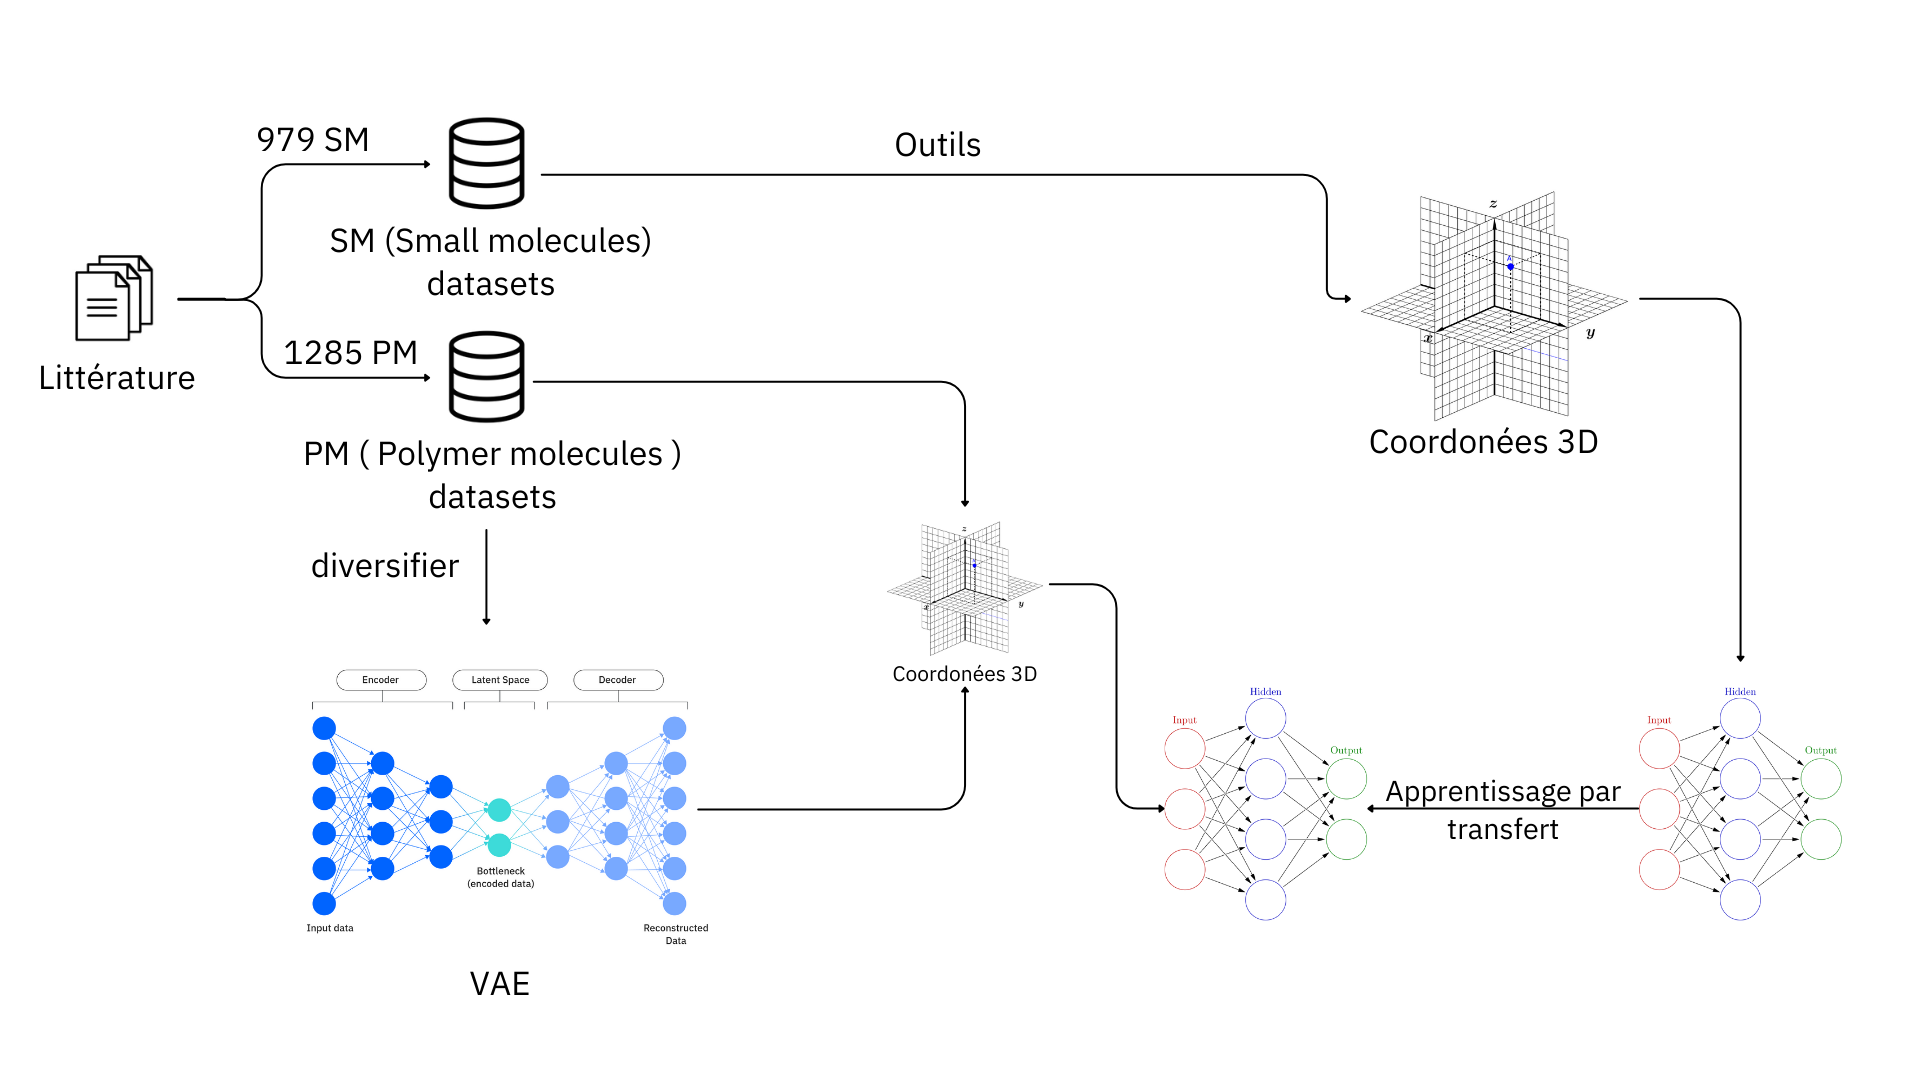
\includegraphics[width=0.8\textwidth]{Architecture/global.png}
    \caption{Architecure globale du modèle}
\end{figure}

On peut voir sur le modèle qu'il y a une série d'étape pour notre achitecture :
\begin{itemize}
    \item \textbf{Tranformations des molécules en 3D} : La première chose à faire est de transformer les molécules en coordonnées pour l'entrainement du modèle.
    \item \textbf{Entrainement du modèle QDF-SM} : Entrainer dans un premier le modèle sur les molécules SM tranformées.
    \item \textbf{Transfert Learning du modèle QDF-PM} : Faire de l'apprentissage par transfert sur les molécules PM tranformées.
    \item \textbf{Génération de molécules} : Génération de nouvelles molécules qui sont à tester sur les modèles entrainés (pour la prédiction).
\end{itemize}

En résumé, l’architecture proposée combine un modèle génératif basé sur un Auto-Encodeur Variationnel (VAE) pour la création de nouvelles structures moléculaires et un modèle de prédiction de propriétés (Quantum Deep Field) pour évaluer leur efficacité photovoltaïque. 
Cette approche intégrée permet non seulement d’explorer efficacement l’espace chimique à la recherche de nouveaux matériaux donneurs, mais aussi de prédire les propriétés de matériaux tels que le PCE.